\documentclass{standalone}
\usepackage{pgfplots}
\pgfplotsset{width=7cm, compat=1.15}

\begin{document}

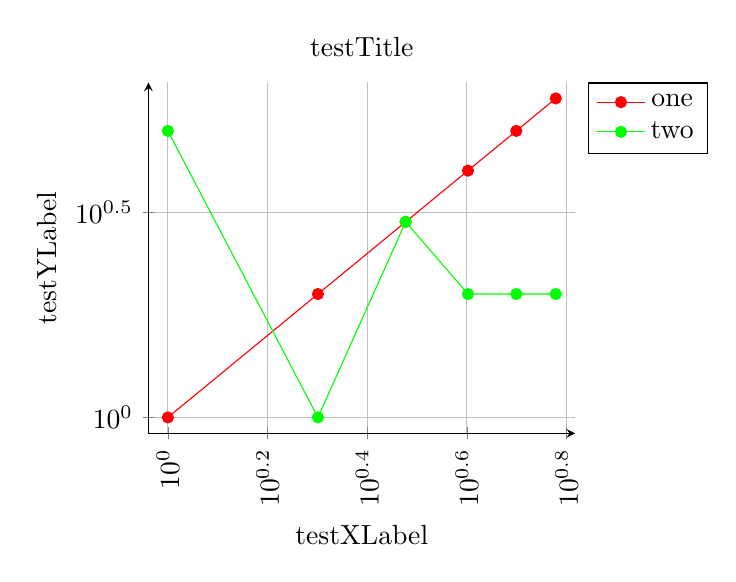
\begin{tikzpicture}
	\begin{loglogaxis}[
		title=testTitle,
		axis lines=left,
		xticklabel style={
			rotate=90,
			anchor=east
		},
		scaled ticks=false,
		xlabel=testXLabel,
		ylabel=testYLabel,
		enlargelimits=0.05,
		grid=major,
		legend entries={one,two},
		legend pos=outer north east
	]

% Coordinates are one pair of x/y coords per line: "(x, y)\n"
\addplot[red, mark=*] plot coordinates {
(1,1)
(2,2)
(3,3)
(4,4)
(5,5)
(6,6)

};
% Coordinates are one pair of x/y coords per line: "(x, y)\n"
\addplot[green, mark=*] plot coordinates {
(1,5)
(2,1)
(3,3)
(4,2)
(5,2)
(6,2)

};

	\end{loglogaxis}
\end{tikzpicture}

\end{document}
